\documentclass[14 pt]{extarticle}

	\usepackage[french]{babel}
	\usepackage[utf8]{inputenc}  
	\usepackage[T1]{fontenc}
	\usepackage{amssymb}
	\usepackage[mathscr]{euscript}
	\usepackage{stmaryrd}
	\usepackage{amsmath}
	\usepackage{tikz}
	\usepackage[all,cmtip]{xy}
	\usepackage{amsthm}
	\usepackage{varioref}
	\usepackage{geometry}
	\geometry{a4paper}
	\usepackage{lmodern}
	\usepackage{hyperref}
	\usepackage{array}
	 \usepackage{fancyhdr}
	 \usepackage{float}
\renewcommand{\theenumi}{\alph{enumi})}
	\pagestyle{fancy}
	\theoremstyle{plain}
	\fancyfoot[C]{} 
	\fancyhead[L]{Nom, prénom : }
	\fancyhead[R]{2 juin 2026}\geometry{
 a4paper,
 total={190mm,277mm},
 left=10mm,
 top=20mm,
 }
	
	
	\title{Contrôle Chapitre 2}
	\date{}
	\begin{document}
 

 \subsection*{Exercice 1 (12 points)}
 
 Tracez les symétriques des figures suivantes par rapport à la droite représentée : 

 \begin{figure}[H]
 \center
 
\includegraphics[scale=.7]{Fig1}
 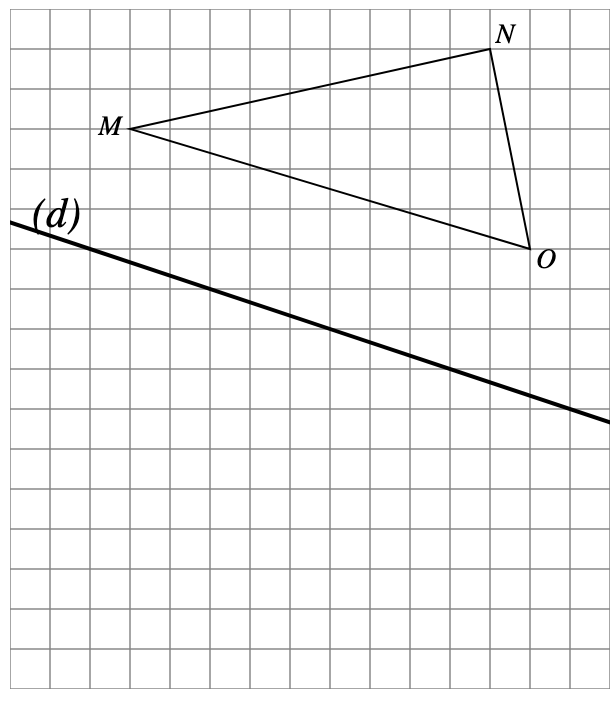
\includegraphics[scale=.7]{Fig2}
 \end{figure} 
  \begin{figure}[H]
 \center
 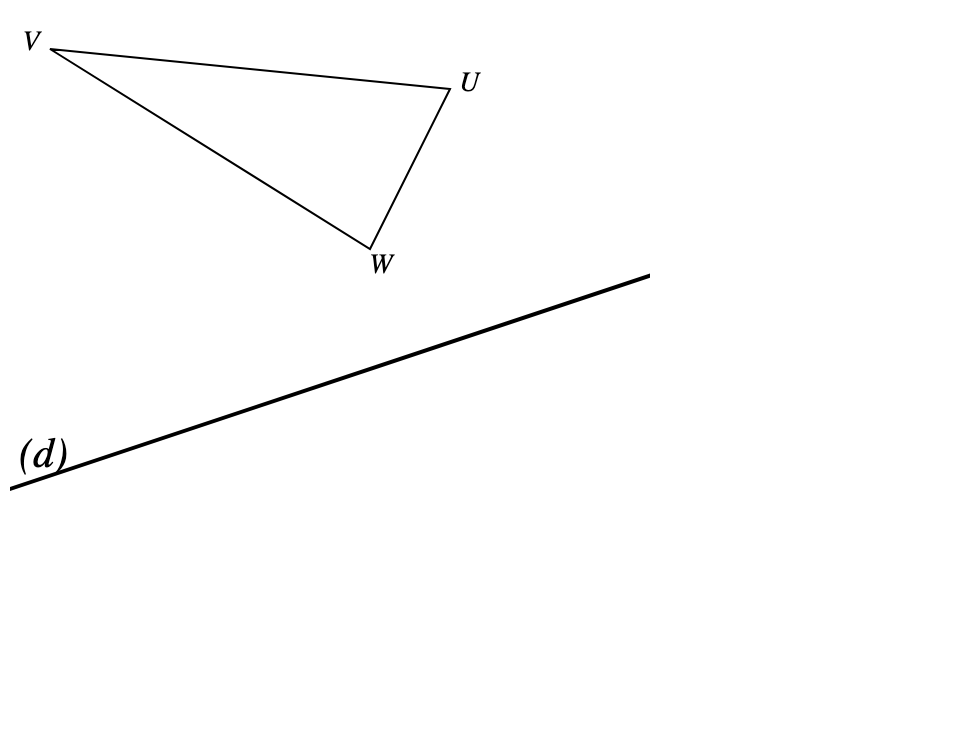
\includegraphics[scale=.55]{Fig4}
 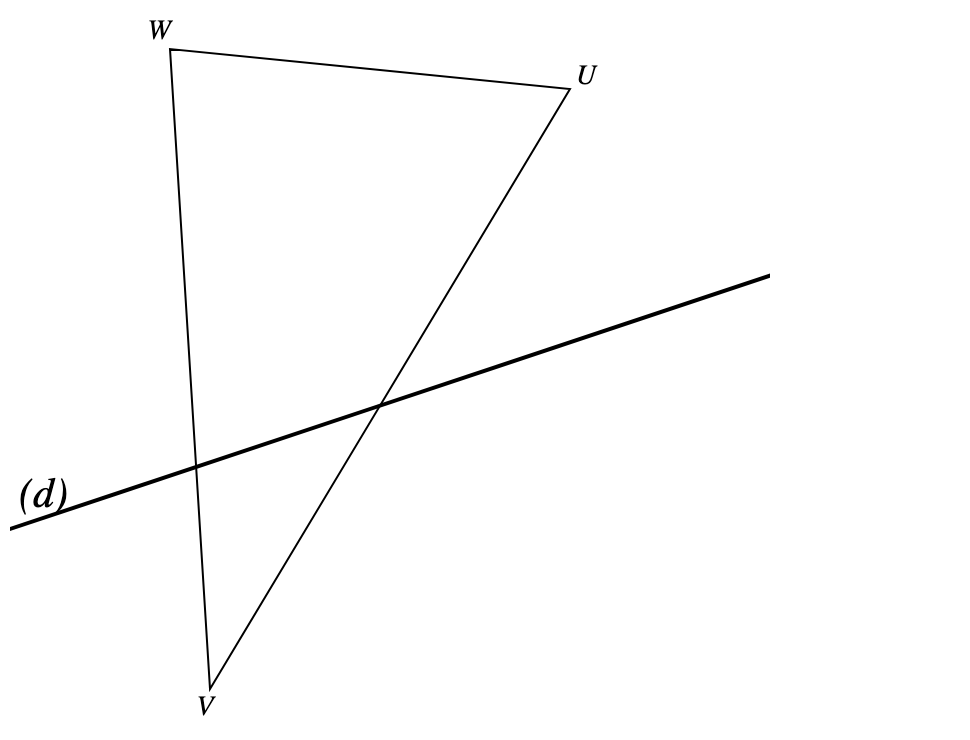
\includegraphics[scale=.55]{Fig3}
 \end{figure}
  \begin{figure}[H]
 \center
 
\includegraphics[scale=.6]{Exo6} 
 \end{figure}
 
 
\subsection*{Exercice 2 (3 points)} 

Sur les figures suivantes, représentez les axes de symétrie éventuels, et dites leur nombre.  

\begin{figure}[H]
\center 

\includegraphics[scale=.06]{Niger.png}\ \ \ \ \ 

\includegraphics[scale=.06]{Suisse.png}\ \ \ \ \ 

\includegraphics[scale=.06]{Honduras.png}
\end{figure}

\subsection*{Exercice 3 (3 points)}  
Soit $ABC$ un triangle isocèle en $A$. 
\begin{enumerate}
\item Notons $I$ le milieu de $[BC]$. Démontrer que $(AI)$ est la médiatrice du segment $[BC]$. 
\item Que dire des points $B$ et $C$ par rapport à cette droite ? (Justifier).
\item Justifier que $(AI)$ est un axe de symétrie de $ABC$.
\end{enumerate}
 
 






 	\end{document}
